\section{Implementation}\label{sec:impl}
The proof of concept was implemented in MATLAB with separate encode and decode stages.
The encode stage takes an image file and a watermark phrase and outputs a watermark embedded image.
The decode stage takes the watermarked and original images and outputs the extracted watermark message.

\subsection{Encoding}
\begin{figure}[tbph]
  \centering
  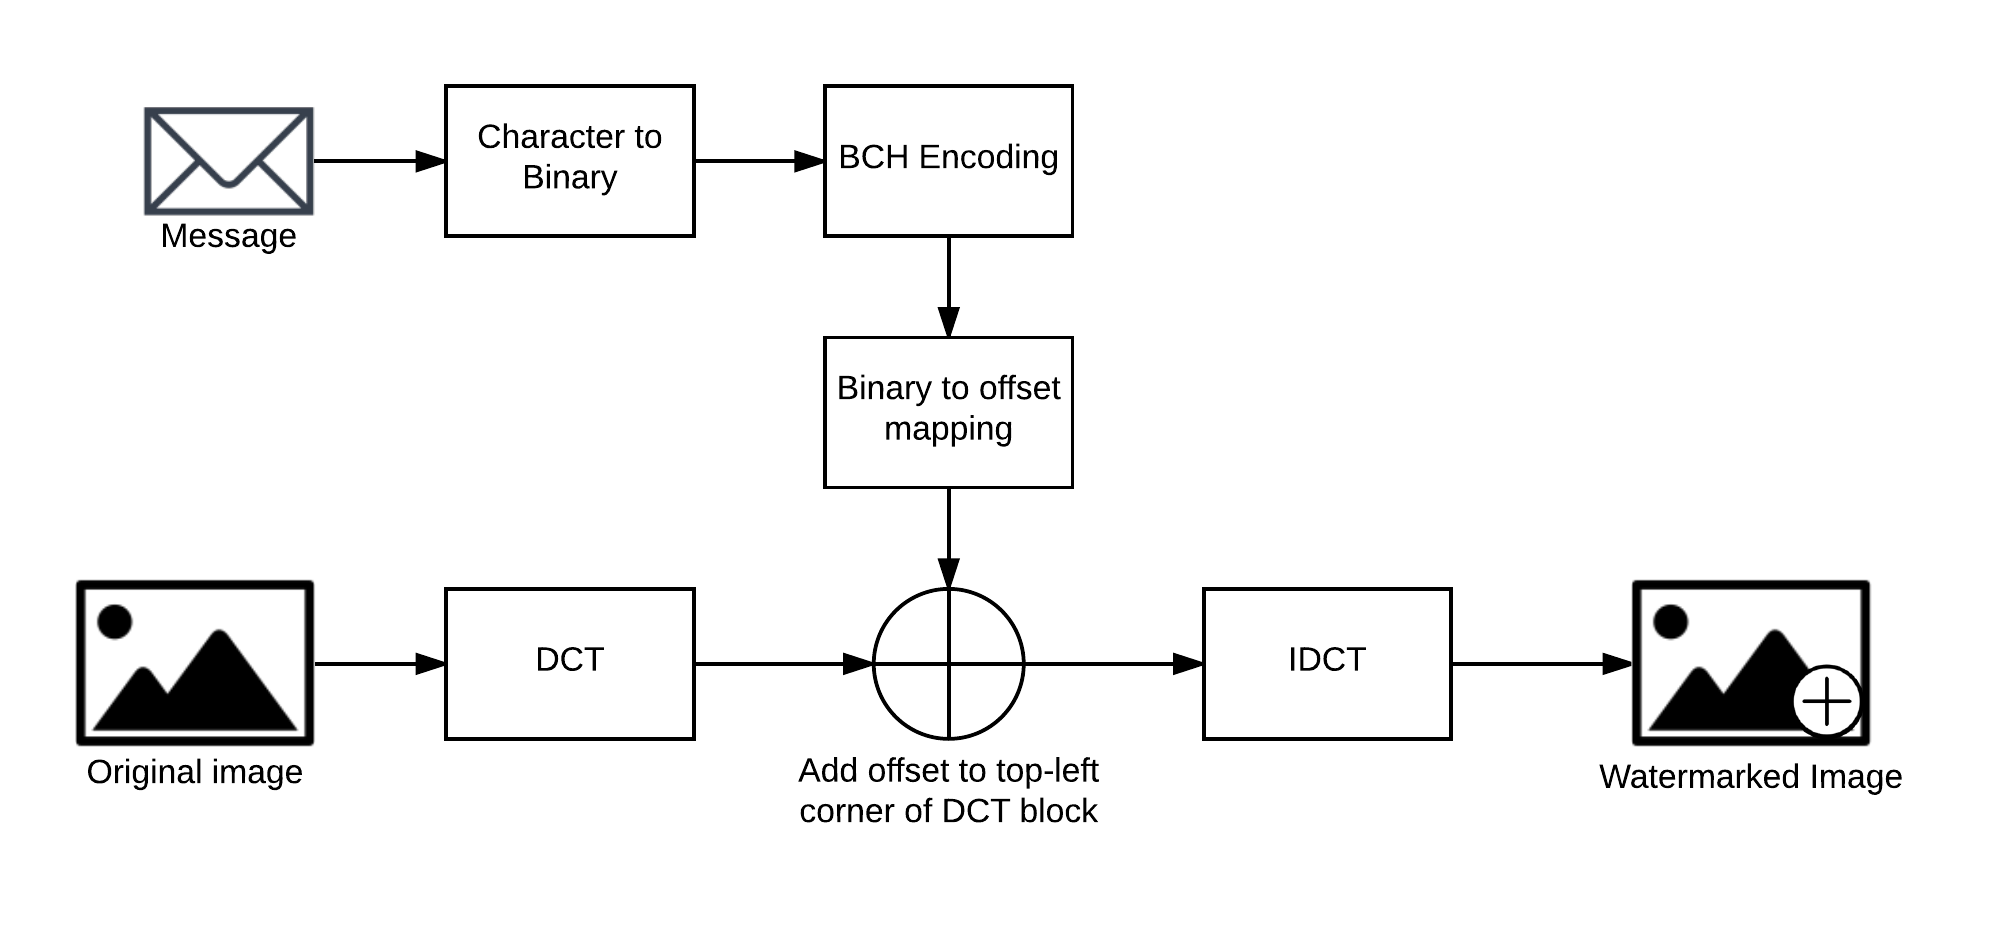
\includegraphics[width=0.75\linewidth]{graphics/encode}
  \caption{Watermark encoding process}
  \label{fig:encode}
\end{figure}

Figure~\ref{fig:encode} shows the encoding process.
The encode file prompts the user to supply a source image and message to embed.
The message must be in basic alphanumeric format and the length is limited to 33 characters as a requirement for the BCH code.

The letters of the watermark message are associated with a number corresponding to its frequency in the English language.\footnote{See: \url{https://en.wikipedia.org/wiki/Letter_frequency}}
This ensures that letters the most frequent letters will have more 0s, and thus a smaller distortion, when mapped onto the source image.
The numbers are converted into 6-bit binary values\footnote{The inclusion of letters \textit{and} numbers in the watermark character space pushes the total number of characters over 32, thus requiring 6 bits.} and form a binary sequence.

The $DCT~\rightarrow~IDCT~\rightarrow~cast~to~\texttt{uint}$ process is \textit{lossy}, primarily because of the downcast to \texttt{uint}.
To minimize ambiguous downcasting we use an offset generation mapping $x \mapsto y$ and recovery mapping $ y^{\prime} \mapsto x^{\prime}$ defined as:
\begin{align*}
y_i = \begin{cases}
0, & x_i = 0\\
2, & x_i = 1
\end{cases}
&&
x^{\prime}_i = \begin{cases}
0, & y^{\prime}_i \le 0 \\
1, & y^{\prime}_i > 0
\end{cases}
\end{align*}

Despite this precaution, recovery errors occur with a rate $\approx 1\%$.
In order to correct this, we apply a BCH code to the binary sequence to allow for error detection and correction.
We use a BCH code with $n = 255$, $k = 199$ capable of correcting 7 errors (2.7451\% error rate).
To apply the BCH code, we pad the binary watermark sequence with 0s so it has 199 bits.
The BCH encoder returns a sequence of 255 bits that can now be embedded into the image.

Next, we obtain the $8\times8$ block DCT of the image.
Each binary value is mapped to the appropriate offset and added to the DC component of the DCT block, starting with the top left block.
Once all 255 bits have been added to the DCT blocks, the image is reconstructed via Inverse DCT and written to an output file.

\subsection{Decoding}
\begin{figure}[tbph]
  \centering
  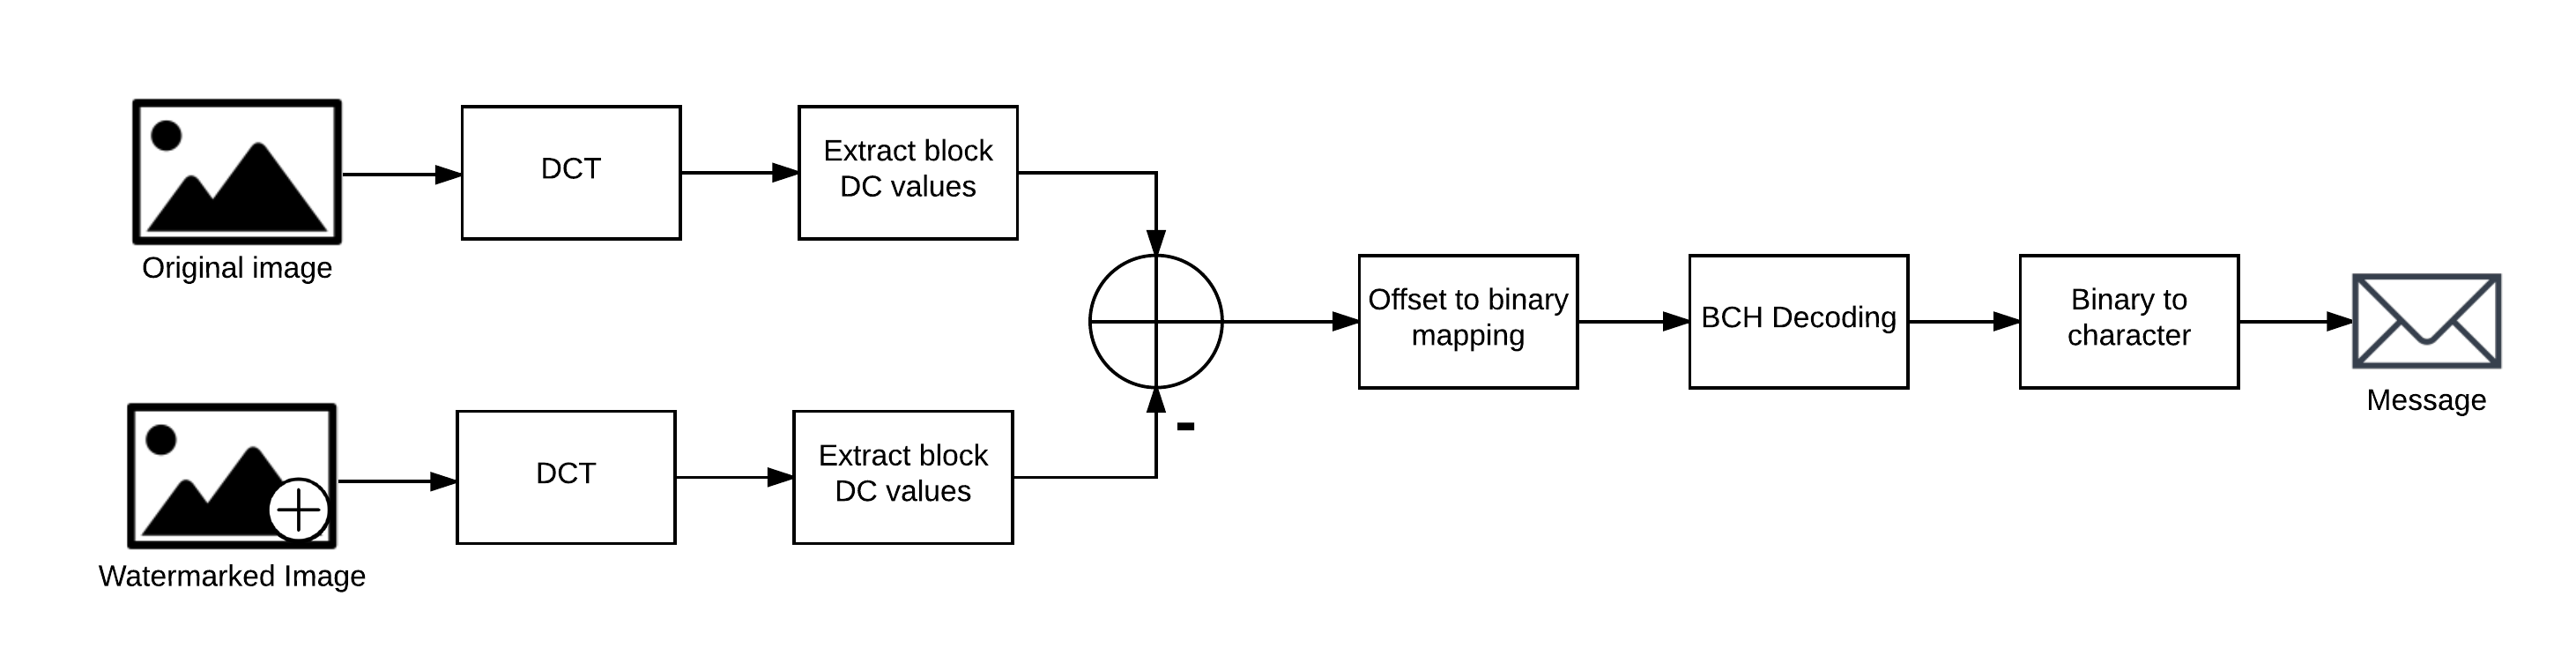
\includegraphics[width=0.95\linewidth]{graphics/decode}
  \caption{Watermark decoding process}
  \label{fig:decode}
\end{figure}

Figure~\ref{fig:decode} shows the process for retrieving the watermark message from the image.
This process is not ``blind'' since it requires the original image to extract the offset values in DCT DC coefficients.
Moreover, the values of $n$, $k$ for the BCH code and the structure of the character-to-binary map \textit{must} be shared by the encode and decode processes.

After recovering the binary sequence, 6-bit words are mapped to their original characters with padding characters mapping to \texttt{" "} empty space.
The user is presented with the extracted watermark.
